
Uma máquina de corrente contínua pode funcionar tanto como um gerador, convertendo energia mecânica em energia elétrica, quanto como um motor, convertendo energia elétrica em mecânica. Apesar de a energia elétrica ser comumente distribuída (no nível do consumidor) em corrente alternada, os motores de corrente contínua possuem grande participação na indústrias, uma vez que permitem facilmente a variação de velocidade, por exemplo, de uma esteira ou um comboio. 

Por outro lado, componentes eletrônicos de tensão alternada, cada vez mais acessíveis, são capazes de controlar a velocidade de motores assíncronos da mesma forma, logo, pelo seu melhor custo benefício, eles vêm substituindo os motores de corrente contínua na maior parte das aplicações. De toda forma, o estudo dos motores de corrente contínua é fundamental pois introduz os conceitos básicos do funcionamento de máquinas elétricas. A figura \ref{fig:MCC} mostra esquematicamente uma máquina de corrente contínua elementar.

\begin{figure}[ht!]
\center
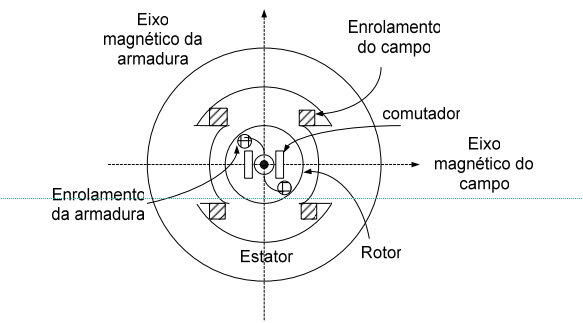
\includegraphics[scale=0.66]{imagens/maquina_cc.png}
\caption{\label{fig:MCC}Máquina de corrente contínua elementar.}
\caption*{Fonte: Máquinas de corrente contínua \protect\footnotemark}
\end{figure}

\footnotetext{Disponível em: <http://www.gsep.ene.unb.br/osem/ivan/Conversao> Acesso em out. 2018.}

